\section{Fanny Shafira Damayanti (1174069)}
\subsection{LeafletJS dan Mapproxy}
\begin{enumerate}
    \item Langkah pertama yaitu run terlebih dahulu mapproxy nya.
  \hfill\break
  \begin{figure}[H]
  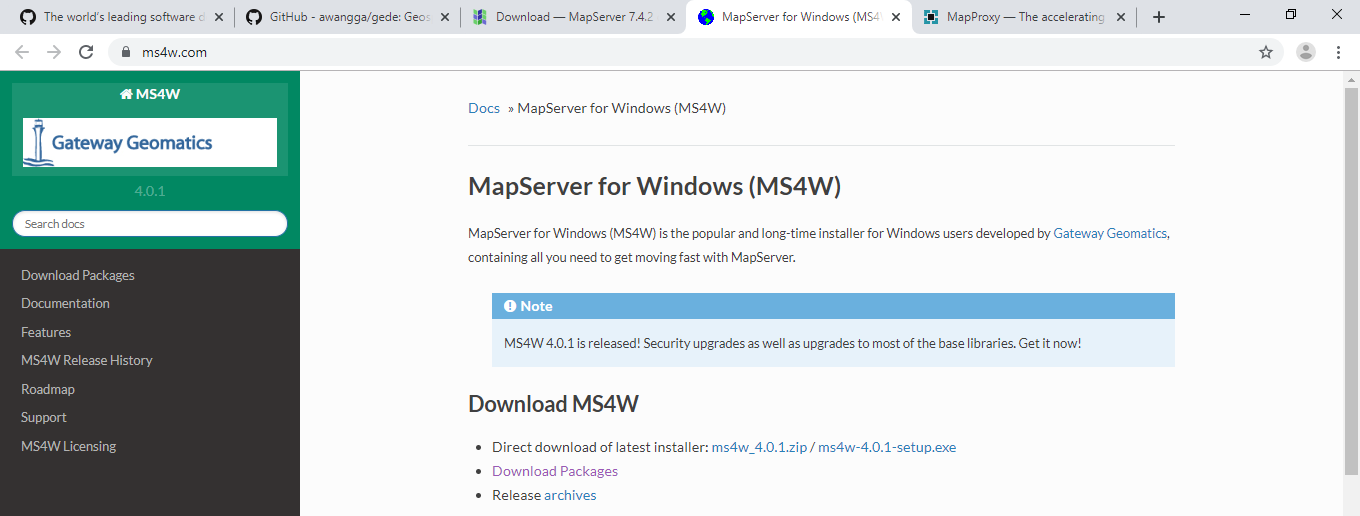
\includegraphics[width=4cm]{figures/tugas5/1174069/1.png}
  \centering
  \caption{Run Mapproxy}
  \end{figure}
    
   

    \item Setelah itu buka contoh file leafletjs yang ada di dalam folder gede  yang telah kita download sebelumnya .
    
  \hfill\break
  \begin{figure}[H]
  
\includegraphics[width=4cm]{figures/tugas5/1174069/2.png}
  \centering
  \caption{Isi Basic.html}
  \end{figure}
    
    \item Kemudian buka browser, maka hasilnya akan seperti ini
    
  \hfill\break
  \begin{figure}[H]
  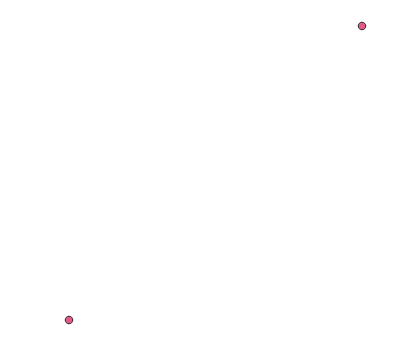
\includegraphics[width=4cm]{figures/tugas5/1174069/3.png}
  \centering
  \caption{Hasil dari Basic.html}
  \end{figure}
  
   \item Dengan menggunakan LeafletJS kita dapat menambhakan marker, circle dan polygon yaitu dengan cara seperti gambar dibawah ini, contoh ini diambil dari file marker.html yang berada didalam folder gerede.
    
  \hfill\break
  \begin{figure}[H]
  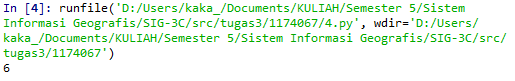
\includegraphics[width=4cm]{figures/tugas5/1174069/4.png}
  \centering
  \caption{Isi dari marker.html}
  \end{figure}
  
   \item kemudian buka filenya di browser, hasilnya seperti gambar dibawah ini.
  \hfill\break
  \begin{figure}[H]
  
\includegraphics[width=4cm]{figures/tugas5/1174069/5.png}
  \centering
  \caption{Isi dari marker.html}
  \end{figure}

\end{enumerate}

\subsection{Link Youtube MapProxy dan Menjalankannya}
\verb|https://youtu.be/j_zLb519AQ0|